\documentclass[a4paper,11pt,fleqn,dvipsnames,oneside,openright]{memoir} 
\usepackage[export]{adjustbox}
\usepackage{tabu}
\usepackage{Preamble}
\usepackage{graphicx}
\usepackage[bottom]{footmisc}
\usepackage[demo]{graphicx}
\usepackage{caption}
\usepackage{subcaption}
\usepackage{graphicx}
\usepackage{titling}


\setlength{\droptitle}{-5em}


\newcommand{\forceindent}{\leavevmode{\parindent=1em\indent}}

\addbibresource{references.bib} %Tilføjer kildeliste

\date{}
\begin{document}

\begin{center}

\includegraphics[width=9cm]{Logo.png}
\end{center}
\subsection*{Innovation and new technology}

Business Administration and Information Systems, HA(it.) \\
5th Semester exam report\\
Professor MSO: Chee-Wee Tan\\
PhD fellow: Albert Fei Liu\\
Copenhagen Business School 2017/2018\\
Hand in date: 20th December 2017\\
14.7 Normal pages, 33.523 Characters\\

\begin{tabu} to 0.8\textwidth { | X[l] | X[c] | }
   \hline
   \textbf{Name} & \textbf{CBS-Mail} \\
    \hline
   Mads Jørgsholm Bierrings  & mabi15ad@students.cbs.dk \\
    \hline
   Morten Brandt Nilsson  & moni15ac@students.cbs.dk \\
    \hline
   Lukas Akbar Monssen   & lumo15ab@students.cbs.dk \\
    \hline
\end{tabu}
\\\\
Note: all references in this report regarding contents, bibliography, appendix, footnotes, figures, illustrations and tables are clickable. 

\newpage
\tableofcontents*
\thispagestyle{empty}

\mainmatter 

\chapter{Introduction}
In the course Innovation and new technology, innovation is defined as follows: “production or adoption, assimilation, and exploitation of a value-added novelty in economic and social spheres; renewal and enlargement of products, services, and markets; development of new methods of production; and establishment of new management systems. It is both a process and an outcome”.  

With this state of mind, one of the group members came up with an idea of a technological innovation on behalf of his interest in art. In the current market for trading art, many opportunities exist but various disadvantages follow each one of them. Together the group collaborated on further development of this idea and created the concept of Artion together.

Artion is an online platform for trading art. The application has two purposes. First it seeks to provide a platform making it quick and easy for private people as well as artists and art-distributors to sell paintings. Secondly, to be an inspiring platform for people who wants to buy paintings. \\

We believe the market is missing a platform combining the two aspects stated above. The current market provides following two models:
\begin{enumerate}
    \item Quick and easy in terms of selling products, but not inspiring in terms of buying products
    \item Time-consuming and difficult in terms of selling products, but inspiring in terms of buying products
\end{enumerate}
We identify an opportunity for Artion by combining the advantages of these two models. This represents the background for initiating the project.\\

In this report we will elaborate and analyse various aspects such as the market environment, potential positioning, value proposition and user tasks. Furthermore, we will clarify our considerations regarding human-computer interaction and explain how data is handled by our vertical prototype. Finally, we will present our business model and enlighten a range of commercial challenges.



\chapter{Market environment}
\label{Market}
\section{Market environment}
Throughout this report, we concern the market for art. In this chapter, we will elaborate the environment of the market to enter, hereby the competitors and the potential positioning of Artion. 

\subsection{Competitors}
The market consists of a wide range of competitors, but we consider respectively Lauritz.com, Bruun Rasmussen, DBA, QXL and various social media platforms to be the greatest and nearest competitors in relation to Artion. The reason why social media also constitutes competition is, among other, due to the increasing popularity in the use of sales groups on Facebook. Furthermore, Instagram has also become a popular channel for sales. 
\\\\
The stated competitors above can be distributed into three groups:

\begin{enumerate}
\item Lauritz.com and Bruun Rasmussen
\item DBA and QXL
\item Facebook and Instagram
\end{enumerate}

As illustrated in appendix \ref{PositioningMap}, group 1 represents a high level of time to market, but a fairly short time spent searching for products. The reason for the high level of time to market, is the extensive process for the seller to create an advertisement. A product must be handed to the company for valuation, picturing, storing and further handling. However, the time spent searching for products (for the potential customers) is quite low, because of the simplicity, consistent content and the time frame on auctions, ensuring there is no abundance of old products on the platforms.\\
\forceindent Group 2 represents a low level of time to market but much time spent searching for products. It is quick and easy to create an advertisement, and there are no requirements in terms of product category, quality and price. This results in an abundance of products. Another issue for this group, which only applies for DBA, is that there is no time frame for the products, contributing to an even greater abundance of old products.\\
\forceindent Group 3 represents a low- to mid level of time to market and much time spent searching for products. Using Instagram for sales purposes is very quick and easy, but this only applies with a lot of followers as a prerequisite. Facebook has a slightly higher level of time to market, as is takes time and might be difficult to find the appropriate sales groups before creating an advertisement. The time spent searching for products (for the customers) for both Instagram and Facebook is high, as it might be very time consuming to find the right groups, hashtags, sites etc.

\subsection{Positioning}
In continuation of the above mentioned aspects, we identify a gap in the market, forming an opportunity for Artion. The need we strive to cover is two-sided; the buyer and the seller. The need of the buyer is a consistent, inspirational and user-friendly platform to buy paintings. The need of the seller is a platform that allows quick creation, thus short time to market, of advertisements, which exposes the paintings for sale without getting lost in the abundance of other products. The combination of these two needs represents the foundation for Artion. The way in which the application will meet these needs, is further elaborated in chapter \ref{ValueProposition}. Currently at DBA, there are more than 15.000 advertisements in the category "Paintings"\footnote{https://www.dba.dk/til-boligen/kunst-og-antikviteter/malerier/}, and we are very certain that a large proportion of these advertisements are due to the lack of a better and more inspirational platform. Furthermore, there seems to be an increasing interest in art among the danish population, with an increase of more than 1 million visitors to the danish art museums in the years 2010-2016, illustrated in appendix \ref{Visitors}. This trend might indicate a growth in the market for art. These, among others, are reasons for our choice of positioning, illustrated in appendix \ref{PositioningMap}.

\chapter{Value proposition}
\label{ValueProposition}
In order to clarify the value proposition of Artion, following sections describe the features and the impact, the proof substantiating the value proposition and the costs we expect related to the launch of the application. The value proposition can be summarised as; easy to market, inspiring to buy. 
\section{Capability}
\subsubsection{Frame recognising camera}
\label{FrameCamera}
The frame recognising camera is one of the essential features that makes our application unique. When a user creates an auction, he must use the built-in camera function that recognises the frame of the painting and only captures what is within the frame. In this way we ensure a consistent presentation of all auctions. This process is illustrated in figure \ref{CreateAuction}.

\subsubsection{Simplicity}
One of the reasons for us to develop this app, is that the existing platforms at the current market are not simple and easy to use. Lauritz.com provides a quite easy and simple application. They manage all of the auctions, including valuation, picturing, storing in showrooms and distribution of products after hammering. We think Lauritz.com provides a simple and easy to use application, but the associated processes are very difficult for both the seller and the buyer, in terms of handling and pickup. 

\subsubsection{Safe transactions}
With inspiration from services like AirBnB and Uber, we introduce the transaction-confirmation feature. All transactions and payments are managed by the application. When an auction has ended, the payment is locked in the system. The seller will be notified when the buyer has payed for the product, but the seller will not receive any money before the painting is received by the buyer. We have implemented an interface that enables the buyer and seller to confirm that the exchange of the product has taken place, whereafter the seller receives the money.  
\section{Impact}
We think too many potential profitable paintings at DBA among other platforms are disappearing in the abundance of products. Currently at DBA in the category "Paintings" we find almost 13.500 advertisements\footnote{https://www.dba.dk/til-boligen/kunst-og-antikviteter/malerier/}. Most of these advertisements does not get any attention and ends up being lost in the crowd. Our application aims to bring them into the light, which it does in three ways; frame recognising camera, simplicity and seven days before expiration.\\ 
\forceindent The majority of the advertisements for paintings at DBA and QXL have really bad pictures, which results in less attention. Examples of the pictures and the presentation of advertisements at DBA and QXL, are illustrated in appendix \ref{CompetitorsPlatforms}. The frame recognising camera feature ensures the picture of a given painting is perfectly scaled and hereby presented in the best possible way. Another issue at DBA is that it does not by default sort the products by the expiration date, meaning the old and "bad" advertisements gets a bad location. \\

Artion benefits the market by providing a platform that makes it easy and quick to create advertisements with consistent and perfectly scaled pictures. Hereby ensuring equal spotlight for all advertisements by always sorting by expiration date and time. 
\section{Proof}
The primary evidence substantiating the value proposition of Artion, is the success of the existing platforms, from which we combine various fragments. The three major concepts we combine are as follows: 
\begin{enumerate}
    \item DBA: Quick and easy to create advertisements (short time to market)
    \item Lauritz.com: Consistent presentation of auctions and 7 days before expiration
    \item Instagram: User profiles with infinite scrolling 
\end{enumerate}
These are three well-established concepts, that has proven to be popular over many years. We consider the success of these concepts as the evidence substantiating the value proposition of Artion. We combine these concepts in order to meet the latent needs of consumers, who make up for a gap in the market, which is elaborated in chapter \ref{Market}.

\section{Cost}
\label{Cost}
The greatest costs we expect to face in relation to launching the application, are costs related to hosting, data storage, transactions and marketing. Firstly, we need to establish a partnership with a hosting company to take care of all technical aspects regarding hosting, maintenance, support and storing of data. The costs related to hosting is dependent on the amount of users, auctions, transactions and so fourth. Furthermore, we need an integration with a payment module, and a subscription for a payment solution. Finally, we need to invest in marketing the application and raise attention in order to attract users. The primary channel we plan to use for marketing is social media, hereby sponsored campaigns. 

\chapter{Value adding activities}
This chapter provides a detailed depiction of the value adding activities being performed by our application. Following sections will explain the activities we consider the most value-adding. The complete range of activities for respectively the seller and the buyer is illustrated as service blueprints in appendix \ref{ServiceBlueprint}. The key innovative feature of our application is the combination of the following three activities. 

\section{Display of auctions}
\label{DisplayOfAuctions}
The first essential value adding activity performed by the application, is the display of auctions. The first step in figure \ref{ServiceBlueprintBuyer} is the customer opening the application. This action performed by the user initiates the application to expose a list of auctions. This list is presented as a grid showing large consistent pictures of the various paintings, including date and time of expiration and price. The frame recognising camera feature ensures a consistent presentation of all pictures in the grid. The grid is divided into two columns and has infinite scroll. The grid displaying all auctions in the application is illustrated in figure \ref{AuctionsGrid}.

\section{Easy and short time to market}
One of the most value adding activities performed by the application is the quick and easy way of creating an auction. The second step in figure \ref{ServiceBlueprintSeller} is the seller pressing the + (create advertisement) button. This action performed by the seller initiates the application to open the frame recognising camera. Once the picture is taken, the seller has to provide the information associated with the painting, and then the auction is ready for publishing. The process of creating an auction is illustrated in figure \ref{CreateAuction}. 

\section{Safe transactions}
Another essential value adding activity is the handling of payments. When an auction has ended, the buyer has to pay the hammer price via the integrated payment module. The payment is then locked in the system and only proceeds to the seller when both parties have confirmed the hand-over via the confirmation interface, provided by the application. This concept is inspired by AirBnB\footnote{https://www.airbnb.dk}. The confirmation interface is illustrated in the horizontal prototype in appendix \ref{HorizontalPrototype}.

\chapter{User tasks}
\subsubsection{Getting in touch with the users}

We want to ensure Artion meets the expectations of potential users. If Artion dont manage to meet the expectations, the consumers might reject using the application. In order to meet the users expectations, we intend to initiate a walk-through process in cooperation with potential users. The purpose of a walk-through, is to conduct a list of requirements in terms of meeting their expectations. The first step in the walk-through is to present the log-in interface for the users. From here the users can access the homepage, which contains the grid of auctions (described in section \ref{DisplayOfAuctions}). Screen shots of the vertical prototype are shown in appendix \ref{AppScreenshots}.\\
\forceindent One of the value-adding activities is the creation of auctions, which is presented by the vertical prototype. When a user creates an auction, he have to press the camera icon in the lower right corner, which opens the frame recognising camera. Once the picture is taken, he must type in the information associated with the painting. Finally, the auction is ready for publishing. The steps of creating an auction are illustrated in appendix \ref{TaskFocusedInterface}\\
\forceindent The output we expect from this process, is a discussion resulting in inputs from the users. 

\subsubsection{Comparison}

We have tested a number of other similar applications among the study group. These tests were intended to clarify the level of time to market and ease of use, when using the competitors platforms to create advertisements. From this process we can conclude, that the platforms provided by the competitors varies a lot, in terms of time to market and ease of use. 

\subsubsection{Learning from user tasks}

With the application we leverage on conceptual models from other applications. The purpose is to support what is considered as general user habbts\footnote{\url{https://www.theverge.com/2017/10/31/16579748/apple-iphone-x-review}}. We believe that the process of creating auctions in Artion is very intuitive, as we have simplified the process even more compared to the competitors.

\chapter{Human-computer interaction}
\label{HCI}
The design of Artion is assembled by fragments of other well-known concepts and re-tailored to the extent of Artion’s needs. This approach secures a consistent design for our users as it appeals to their cognitive thinking. The design is also minimalistic as we want the user to think about Artion as a gallery providing the frames for art that speaks for itself.
\subsubsection*{Context}
Different pages of Artion has to connect seamlessly. While one of Artion’s main purposes, is to solve the time-consuming barriers of trading art, the process in navigating through the app should be easy to adapt and remember. Assumptions about how many levels and how many choices pr. Level Is necessary to ensure this. Therefore, as a general contextual design, we want to have few levels and more choices pr. Level.  (see figure. ?)
\subsubsection*{Content}
It should be easy to separate content. Our focal point for value creation starts when users scrolls through the grid with listed art. Since the app is distributing art it’s important that each expression of a product is able to be captured. Therefore, the art becomes the frames of each item in the grid. Another key element in the concern of content is, that it should be easy to go further if the auction being exposed isn’t appealing, therefore the scrolling is continuous and only stops whenever the user selects an auction, or if there are no more auctions in the grid. Same concept as in Instagram. We also want to ensure that the user nor is being distracted by information that isn’t necessary, so the user will only see information about price and time left for the particular auction. This leads to a potential problem because the grid is defined by art uploaded by the users. One way to control this, is to make the user select a standard frame when creating an auction, which makes the whole grid more presentable as it follows one standard. (Various assumption about improving this standard will be described on more details later.)
\subsubsection*{Community \& communication}
To some extend Artion is a community, as it is a focal point for people, with interest in art. However, as Artion only is a demo there won’t be an internal communication system for the users. The community of Artion is expressed in having personal profiles with a gallery of art and an option of searching for other users. 
\subsubsection*{Customisation \& connection}
As mentioned earlier we want to capture only the necessary information. There are many different categories in art and therefore a user should be able to tailor the need of information by sorting for categories. In this way information is restricted to the buyer’s needs. However, one could argue that when Artion is launched it has a low number of users which makes a categorising unnecessary and maybe even frustrating (because of less probability in finding art matching the search criteria).Therefore, filtering for information should follow the level of information exposed. As a start, users will only be able to customise information with a pin-function, where you can follow auctions. (see picture).

\subsubsection*{Commerce}
Commerce is vital for the trust between buyers and sellers. Regarding the design, it is important that both buyer and seller is confirmed when an auction is won. see auction won mock-up. Furthermore, it should be visible that a transaction is locked by Artion until the buyer has confirmed the transaction. If the seller does not respond, the transaction will be cancelled and the amount will be reversed to the buyer. To secure trust between buyer, seller and Artion as a third part it’s important that information about every step in this process is accessible. (see diagram for safe transactions)

(same concept as Airbnb)\\

\chapter{Data handling}
In this chapter, we will briefly describe how the application-prototype handles data, including how it displays, saves and loads data. Additionally, we will shortly enlighten how the data should be captured if the application were to go live. 

\section{Data in the prototype}
The database used for the prototype is developed with Firebase\footnote{https://firebase.google.com/}, a real-time database enabling to store and sync data in real-time across all connected clients. The vertical prototype comprises data such as user data, image files, attributes for paintings etc. In terms of authentication, we have only enabled email/password as sign-in provider. The user information is being encrypted. \\

The vertical prototype enables the user to create an advertisement with 'title', 'author' and 'dimensions' as attributes, simultaneously with an image attached. The picture, including the attributes, is then stored in the Firebase database, whereafter it is loaded and integrated into the grid of auctions in the application. The users in the prototype are hard-coded, but the auctions are created through the application. The data structure for auctions in the database consists of one parent layer containing the attributes as child items. 

\section{Considerations on data capturing}
If the application were to go live, data should be captured differently from the vertical prototype we have developed. Firstly, we use dummy data for users, since the prototype is missing an interface for creating users. If the prototype was a complete platform, it should contain an interface enabling new users to create accounts. Furthermore, the pictures attached to the auctions in the prototype are dummy data. In a final product the images should be captured by the previous described frame-recognising camera feature (described in chapter \ref{ValueProposition}). Another aspect we haven't addressed in the prototype is the process, and data exchanged, in terms of bids on auctions. 

\chapter{Business model}
\subsubsection{Value proposition}
Artion is a trading platform and a community that connects interests of buyers and sellers. Upcoming artist often see breaking the barriers as the hardest part as it can be difficult to address their customers. Art-distributers looks for ways to distribute art to customers with a minimum cost to maximise profit. Together both want to access customers with a low cost. As explained in the market analysis there is various ways to promote art but there isn’t a platform that connects everything together. The value proposition of Artion is to connect everything in one application. Artion is not only for trading art, it’s community for creative artist who wants to share ideas and get inspired among profiles of other artist.

\subsubsection{Market segment}
The market consists of people having an interest in art, but with various agendas. We divide the market into three segments; artists, gallerists and private people. The proposition will be appealing in general, because of the ease of use, appealing interface and the inspiring platform. On the other hand, we acknowledge that our users could have various agendas. 
Artion reach both the amateur artist who creates art as a hobby and professionals that makes a living out of it, as Artion handles trading and provides personal profiles which can be helpful in establishment of a name. We also want to reach to the gallerists, but their agenda is usually more focused on making profit, so they might find the low cost of use as the appealing element. At last Artion is appealing to private people because of the easy to market proposition.
This means that the value generating mechanisms can vary and, therefore, Artion serves various purposes. Some might only use it for trading, some might use it to be a part of the community and some might use it for both trading and the community.


\subsubsection{Value chain structure }
Artion’s structure of value chain comes in two categories. As a trading platform and a community. We prospect these two as the reason a buyer would pay for our service.

\subsubsection{Artion as a trading platform}
Artion seek to reduce the barriers of selling art. The cost of selling art is hard to measure because it depends on many variables. For example promotional skills of the artist or art-distributer, the demand for art, popularity and so on. In this matter, we identify three teleological issues; finding an audience, expanding an audience and keeping an audience. If these are supported to an extend where the three segments effort in using the platform, is less the value generated from creating an auction, we believe that there are incentives for using Artion and value can be captured for both our users and Artion. 

\subsubsection{Artion as a community}
We believe that having a community can establish value for our segment. As we identified in our market analysis, many artists distribute art through different medias and platforms. If the trend is to promote art through these, then our trading platform should include a community to support the needs of our segment.\\

When these two connects the market becomes more visible for everyone and thus a decrease in cost of selling art. When this is based on the prospected needs of the market, we identify our segment as our assets needed in order to support our position. Therefore, users are crucial to the value structure of Artion.

\subsubsection*{Cost structure \& profit potential}

As indicated in the value proposition and the structure of value chain we see that users and value is causally connected. Artion charges 4\% in commission for every auction sold through the platform. This identifies Artion’s revenue streams as a retail revenue model, as Artion work as a third part in the transaction of an auction. Both pros and cons follow this type of revenue stream. Pros in the sense of a predictable revenue stream and cons in sense of being projected to appealing product lines, which in this situation can be specific art. 

\subsubsection{Cost expected to occur}
In commercialization of Artion is digital marketing & online advertising, events, support and use of firebase. Cost of development is not taken into account, as we expect to develop the app ourselves. Is hard the measure a budget of these as no truth from historical data from artion exists. However various expectations follow.

\subsubsection{Digital marketing and online advertising}
We expect to prioritize this in the beginning because of the crucial importance of recruiting members. Most providers like google, Facebook Instagram has different scalable solutions so information about this cost obtainable.

\subsubsection{Data storage and Firebase}
When testing our app, we saw that one hour of distributing data between our client and firebase exceeded the 1 GB trail period of firebase. Unfortunately, firebase only tracks 30 days of storage-information, so this information is no more accessible and in lack of user test, this is the only historic-user data to forecast a potential data handling progress. However, this is important in considering pricing plan from firebase. If we can exceed 1 GB data in hour of testing, something might indicate that we are vulnerable for burst loads. We identify various reason for this occurrence. One is our compression of pictures in react-native. As we use fetch-blob to collect binary data for storage, the sizing of a picture has an impact of big a stored string is, which is directly traceable as a cost in any of the pricing plans. Therefore, we expect to work on a solution that compresses data more efficient in order to lower cost.
\subsubsection{Support and events}
Cost will occur when promoting events and supporting our customers. We expect the cost of support to be a variable cost of users and the cost of events to be fixed.
\subsubsection{Vaue network}


\subsubsection{Competitive strategy}
formulate the competitive strategy by which the innovating firm will gain and hold advantage over rivals. 

 - måske noget om platform thinking og service innovation. Slide 07 og 08

\chapter{Commercial challenges}
In order to prepare for a succesfull entry to the market, we have created a list of commercial challenges. In the sections below we will elaborate the most important challenges, but the complete list of challenges is illustrated in appendix \ref{CommercialChallenges}.

\subsubsection{Gaining market shares}
In a market with strong and well-established competitors, it is difficult for a new company to gain a market position. Companies such as Lauritz.com, Bruun Rasmussen and DBA have existed for several years, and have a strong position in the mind of the consumers. The challenge is to convince the consumers to use Artion instead of the platforms they are used to.\\
\forceindent With our analysis of the competitors business models in appendix \ref{BusinessModels}, we are aware of entry barriers in the market. We believe we have the needed innovative value proposition in order to penetrate the market.

\subsubsection{Deadlocks}
The second challenge is to eliminate the possibility for a deadlock. The whole foundation for the app is based on the presence of both buyers and sellers. If only buyers are present, the application has no purpose. The same applies for the other way around. The sellers need buyers to purchase the products, and the buyers need sellers to provide products. We need to attract both parties before launching the application, in order to establish this synergy effect. 

\subsubsection{Meeting the needs of each segment}
As described in section \ref{Segment}, we identify three segments for Artion. Confronting all segments at the same time might be very difficult in terms of marketing and strategy. Therefore, we have to develop separate marketing strategies for each segment in order to accommodate their diverse needs. 

\chapter{Conclusion}
Based on the analysis of the current market for trading art, we identified a gap that potentially can generate value. The gap occurs because of the existing trading platforms lack of providing
the necessary service to cover the needs we have identified, for people interested in art. On behalf of this assumption, we utilized software development in order to develop a platform called Artion.\\ 

Artion seeks to meet the market segment by providing innovative features that ensures an easy to market gateway. In order to secure adoption of the application, we designed the interface to support the existing conceptual models from the current platforms used for selling art. In order to commercialise Artion, we conducted a viable business model to mediate between the technical and economic domains. As Artion is still in the development stage, the conducted business model takes starting point in the expected costs and profit to occur when launching the finished product. Furthermore, various strategic considerations regarding establishment of innovation was composed to an overall strategy, in order to obtain competitive advantages. In extension of this, a list of potential commercial challenges was created, for better management of the challenges Artion might meet. In conclusion of the above, we believe that Artion will generate value in a real practical scenario. 

% Kildeliste - brug \cite{} ved henvisning
\begingroup
	\raggedright
	\printbibliography
\endgroup 

% Bilag - brug \ref{} ved henvisning
\appendix

\chapter{Appendix}

\section{Positioning Map}
\label{PositioningMap}
\begin{center}
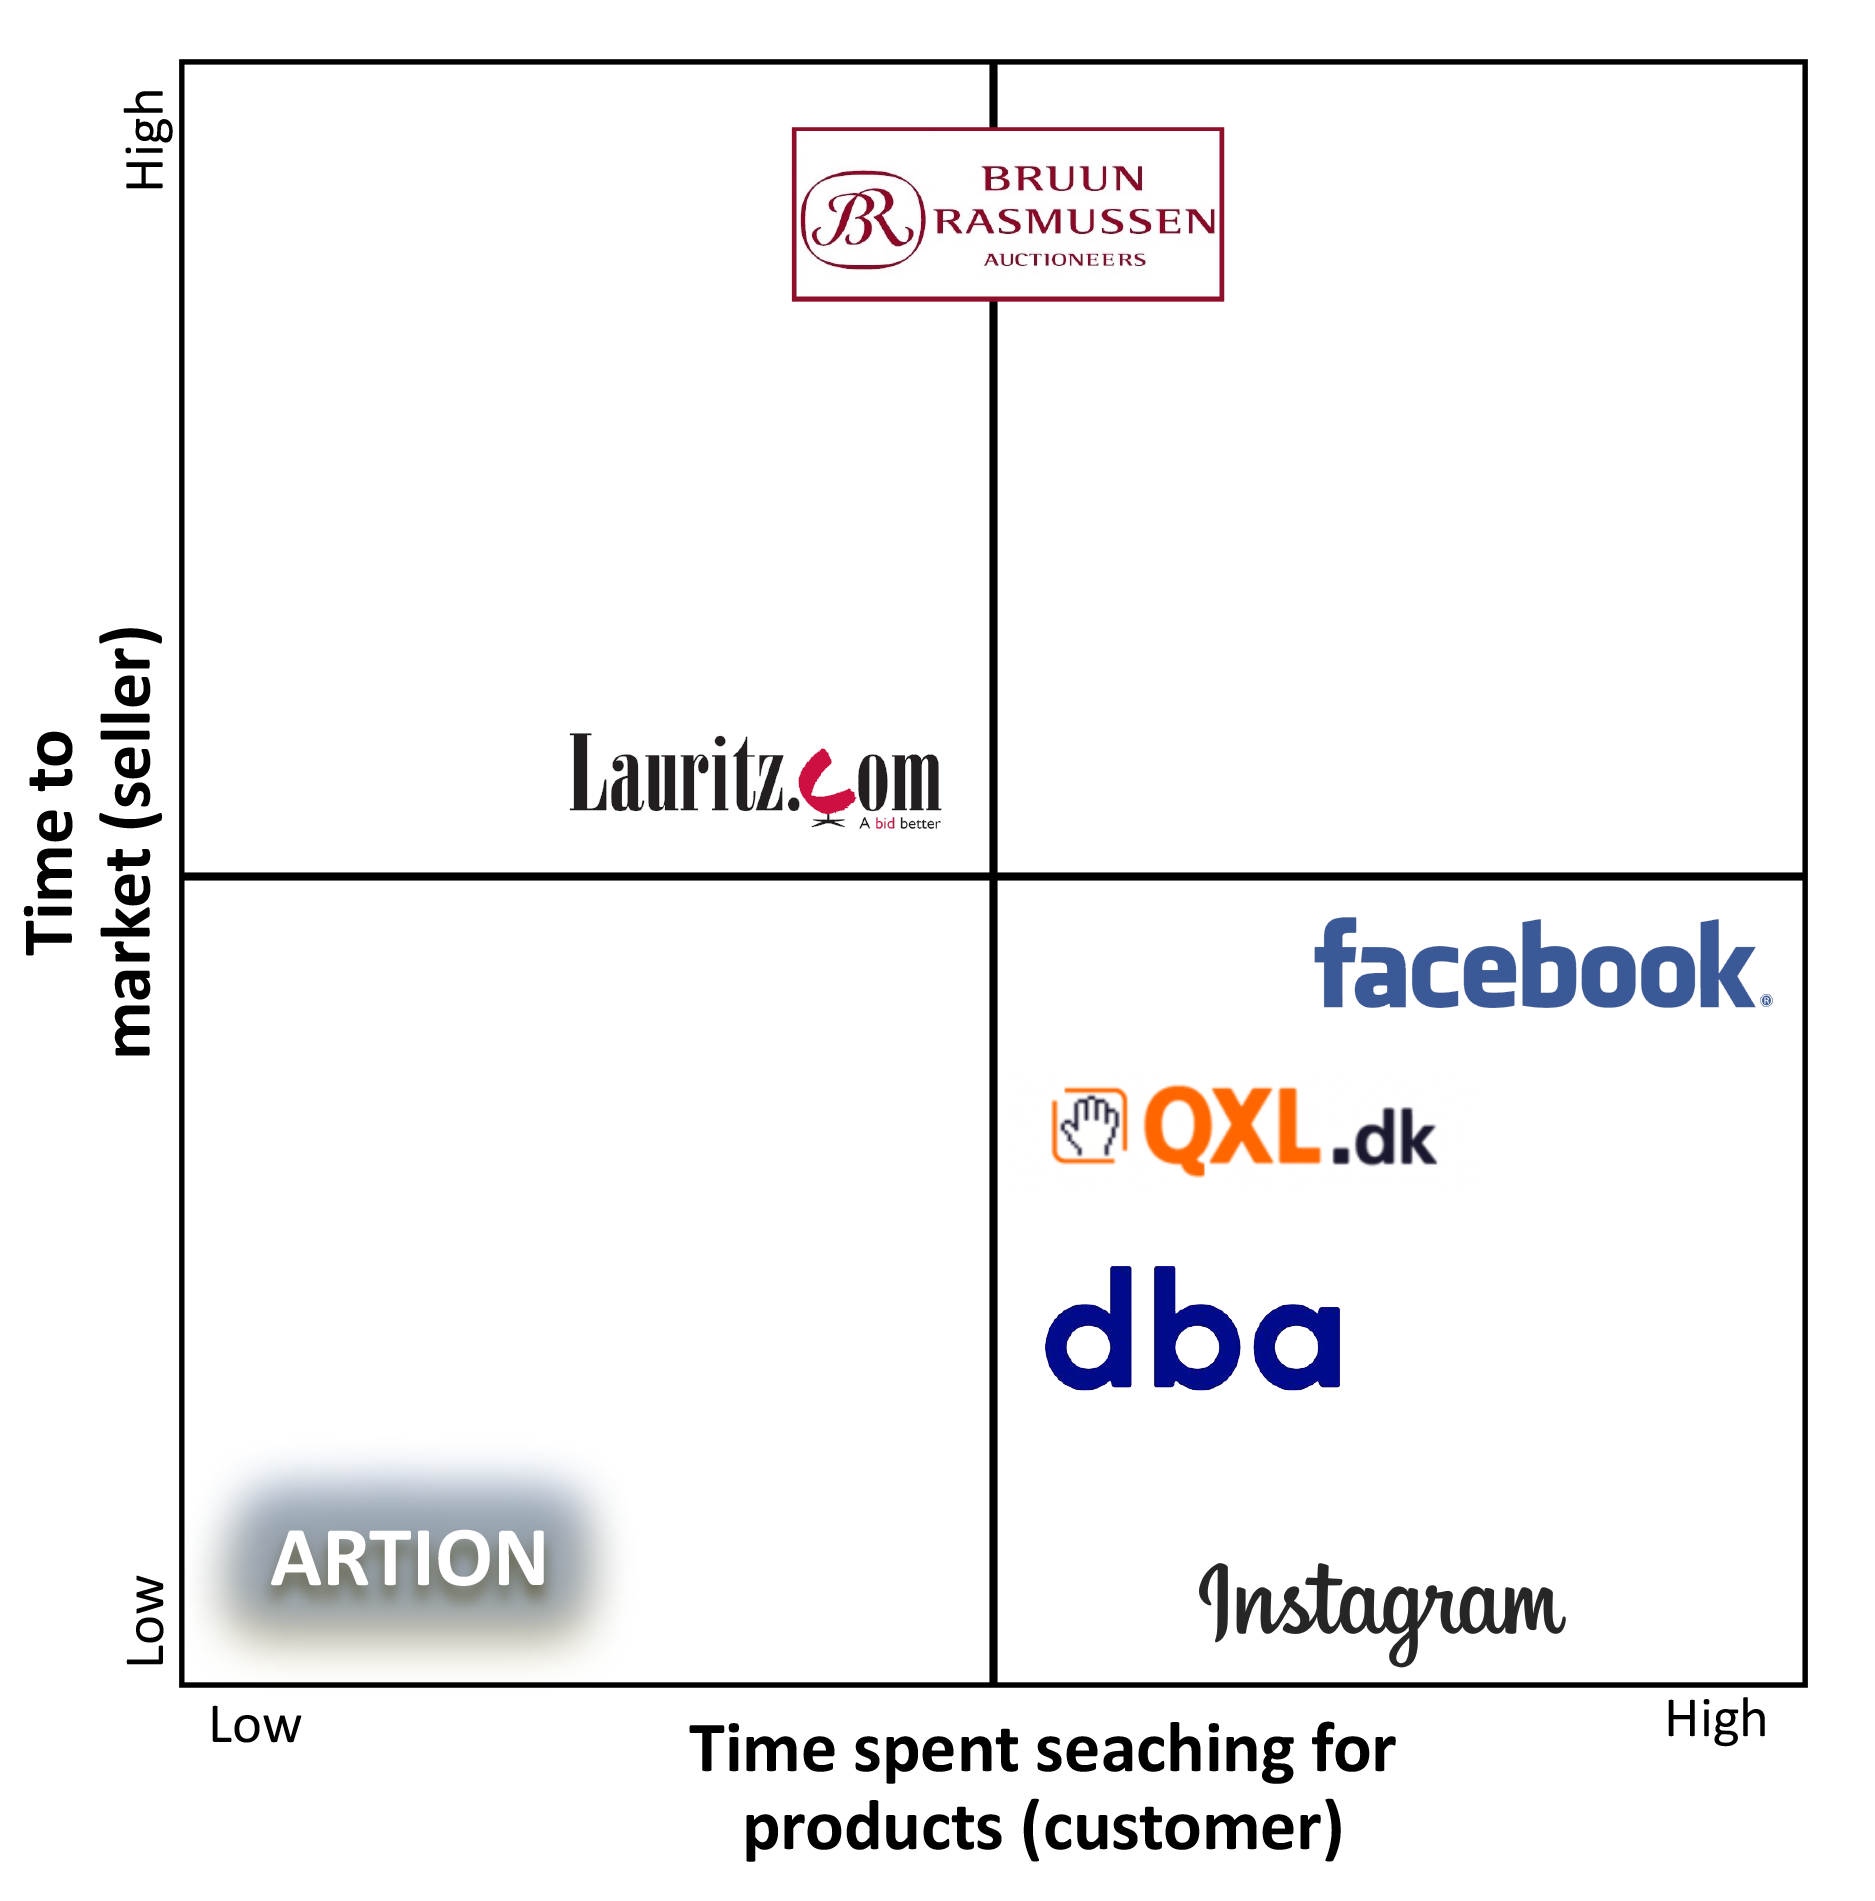
\includegraphics[width=12cm]{Appendix/PositioningMap.png}
\end{center}
\newpage

\section{Visitors at art museums in Denmark}
\label{Visitors}
The data in the table below is based on table MUS1 from Statistics Denmark\footnote{http://www.statistikbanken.dk/10259}.

\begin{center}

\includegraphics[width=16cm]{Appendix/VisitorsArtMuseums.png}
\end{center}
\newpage

\section{Screenshots of competitors platforms}
\label{CompetitorsPlatforms}
\begin{figure}[H]
\centering
  \begin{minipage}[b]{0.285\linewidth}
    \caption{Lauritz display}
    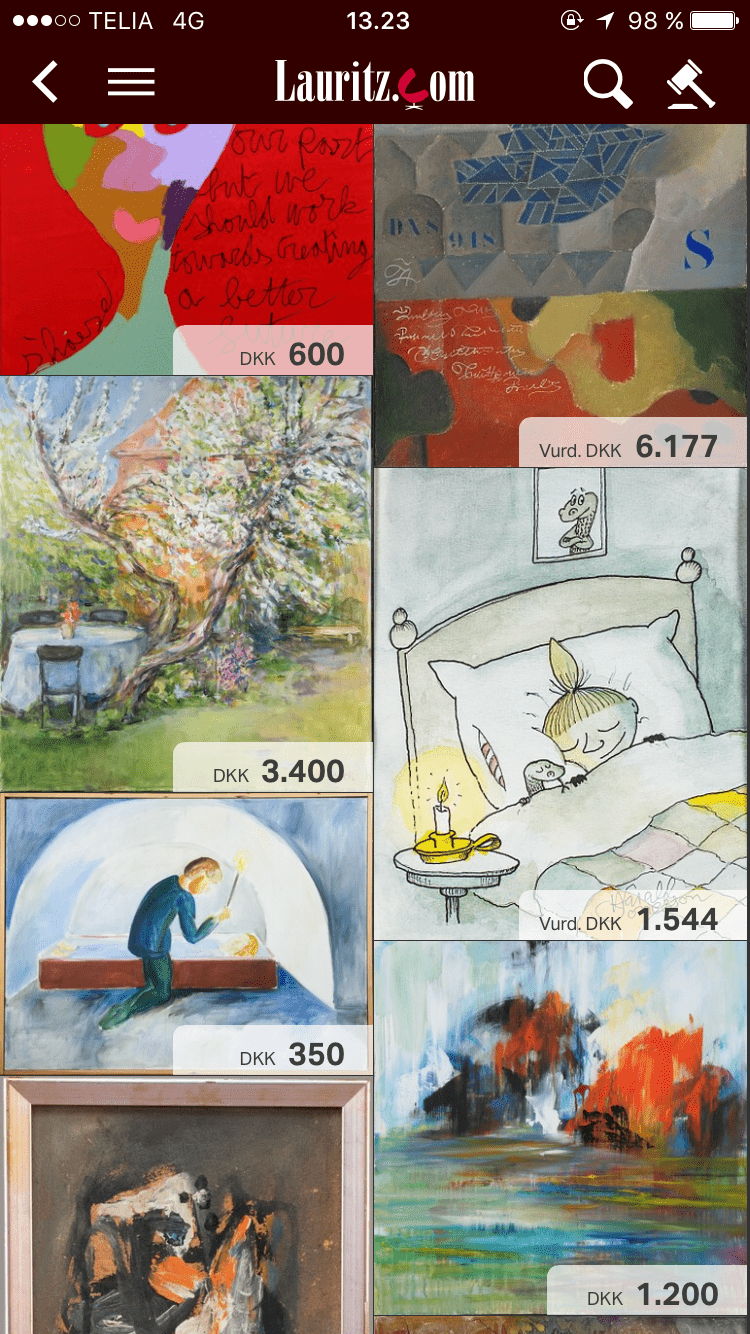
\includegraphics[width=\linewidth]{Appendix/ScreenshotsCompetitorsPlatforms/Lauritz-min.png}
    \label{LauritzDisplay}
  \end{minipage}
  \hspace{0.6cm}
  \begin{minipage}[b]{0.285\linewidth}
    \caption{QXL display}
    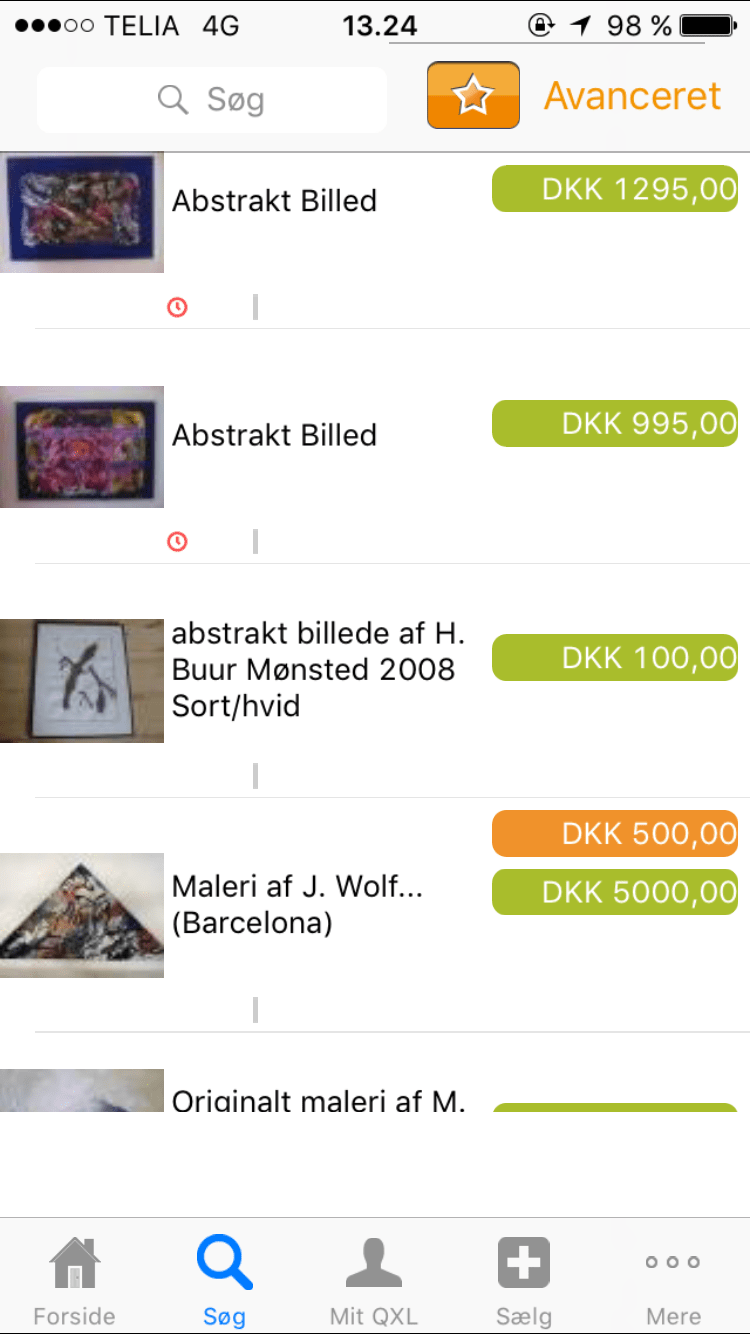
\includegraphics[width=\linewidth]{Appendix/ScreenshotsCompetitorsPlatforms/QXL-min.png}
    \label{QXLDisplay}
  \end{minipage}
 \hspace{0.6cm}
  \begin{minipage}[b]{0.285\linewidth}
    \caption{DBA display}
    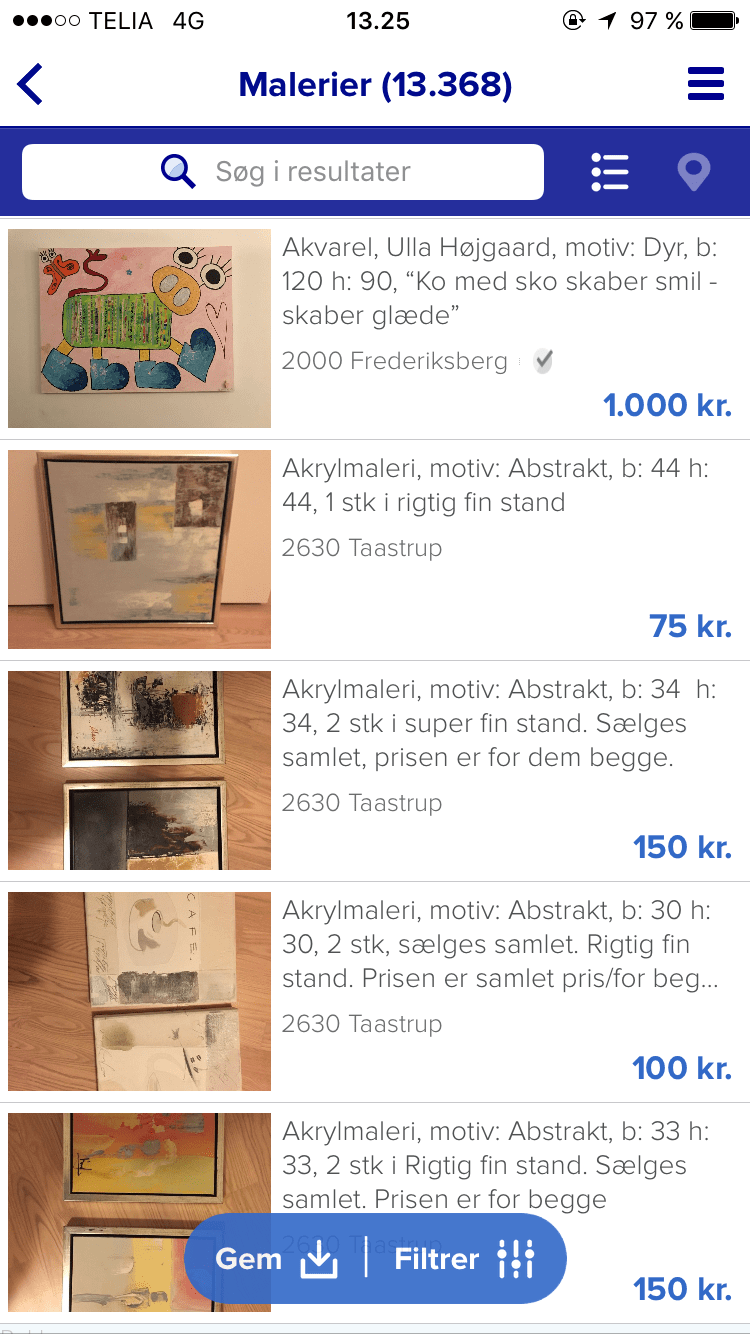
\includegraphics[width=\linewidth]{Appendix/ScreenshotsCompetitorsPlatforms/DBA-min.png}
    \label{DBADisplay}
  \end{minipage}
\end{figure}

\begin{figure}[H]
\centering
  \begin{minipage}[b]{0.285\linewidth}
    \caption{\newline Facebook group}
    
\includegraphics[width=\linewidth]{Appendix/ScreenshotsCompetitorsPlatforms/facebook.jpg}
    \label{FacebookGroup}
  \end{minipage}
  \hspace{0.6cm}
  \begin{minipage}[b]{0.285\linewidth}
    \caption{\newline Instagram profile}
    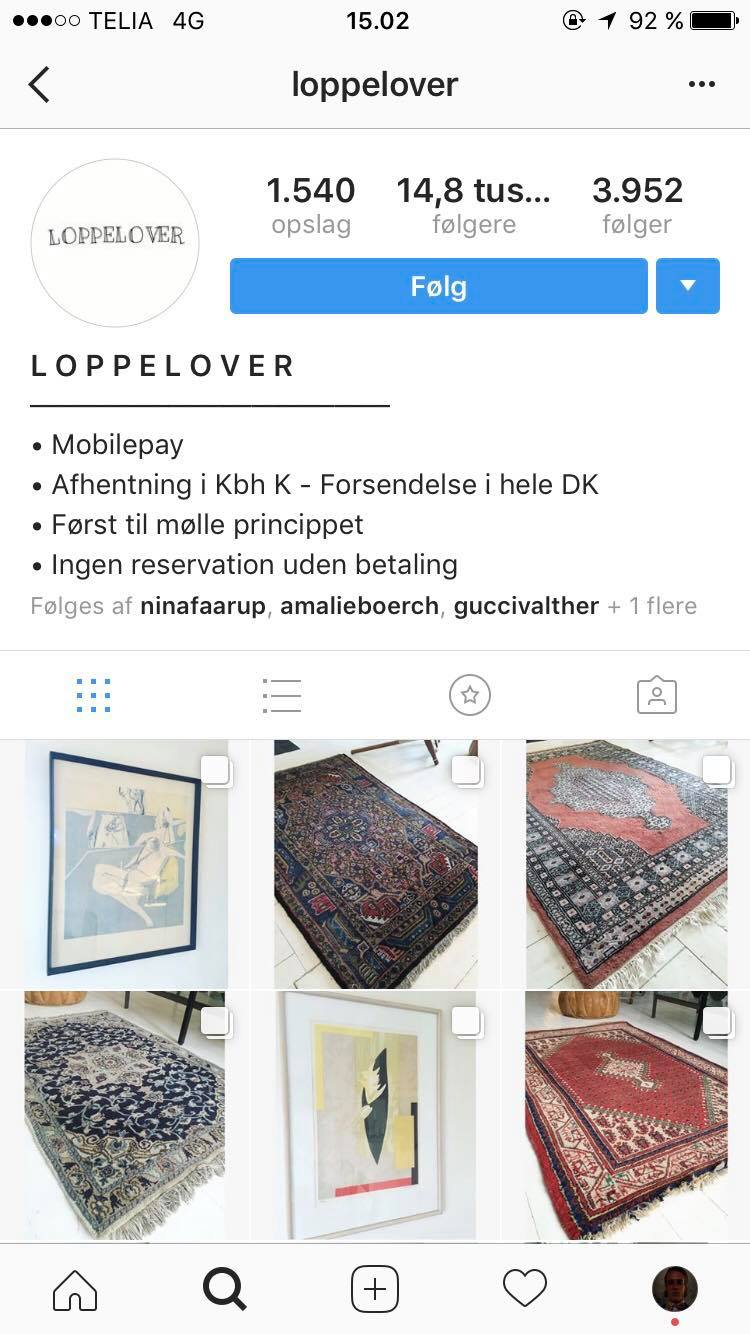
\includegraphics[width=\linewidth]{Appendix/ScreenshotsCompetitorsPlatforms/Instaprofile.jpg}
    \label{InstaProfile}
  \end{minipage}
 \hspace{0.6cm}
  \begin{minipage}[b]{0.285\linewidth}
    \caption{\newline Instagram post}
    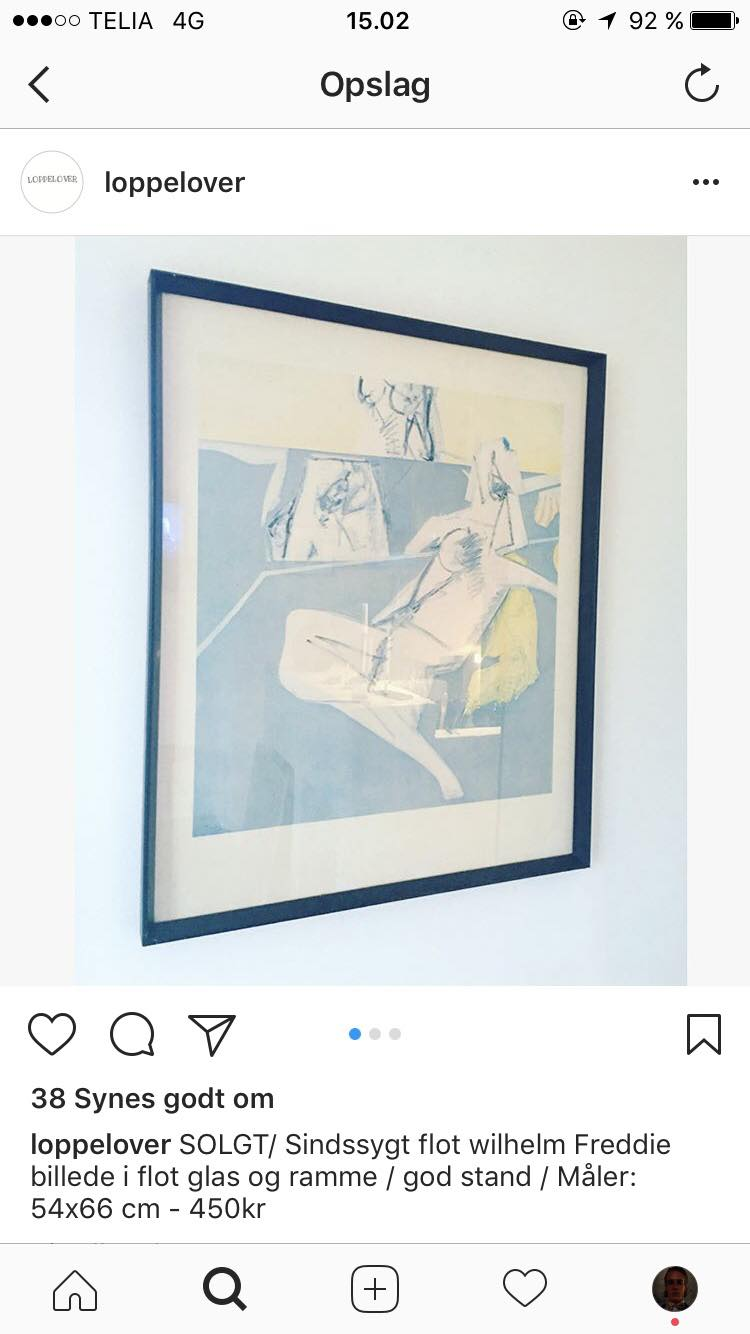
\includegraphics[width=\linewidth]{Appendix/ScreenshotsCompetitorsPlatforms/instapost.jpg}
    \label{InstaPost}
  \end{minipage}
\end{figure}
\newpage

\section{Service blueprints}
\label{ServiceBlueprint}
Service blueprints for the seller and the buyer:

\begin{figure}[H]
    \centering
\caption{Service blueprint for the seller}
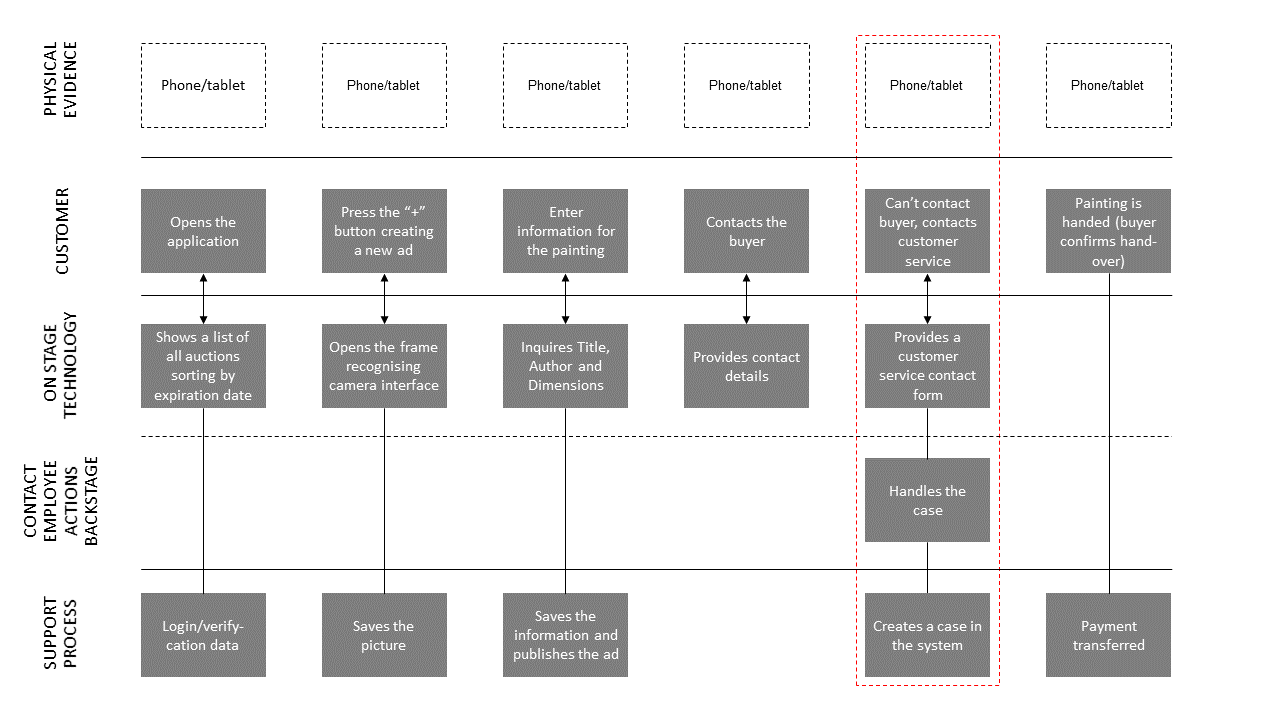
\includegraphics[angle=270,origin=c,width=12cm]{Appendix/BlueprintSeller.PNG}
\label{ServiceBlueprintSeller}
\end{figure}

\begin{figure}[H]
    \centering
\caption{Service blueprint for the buyer}
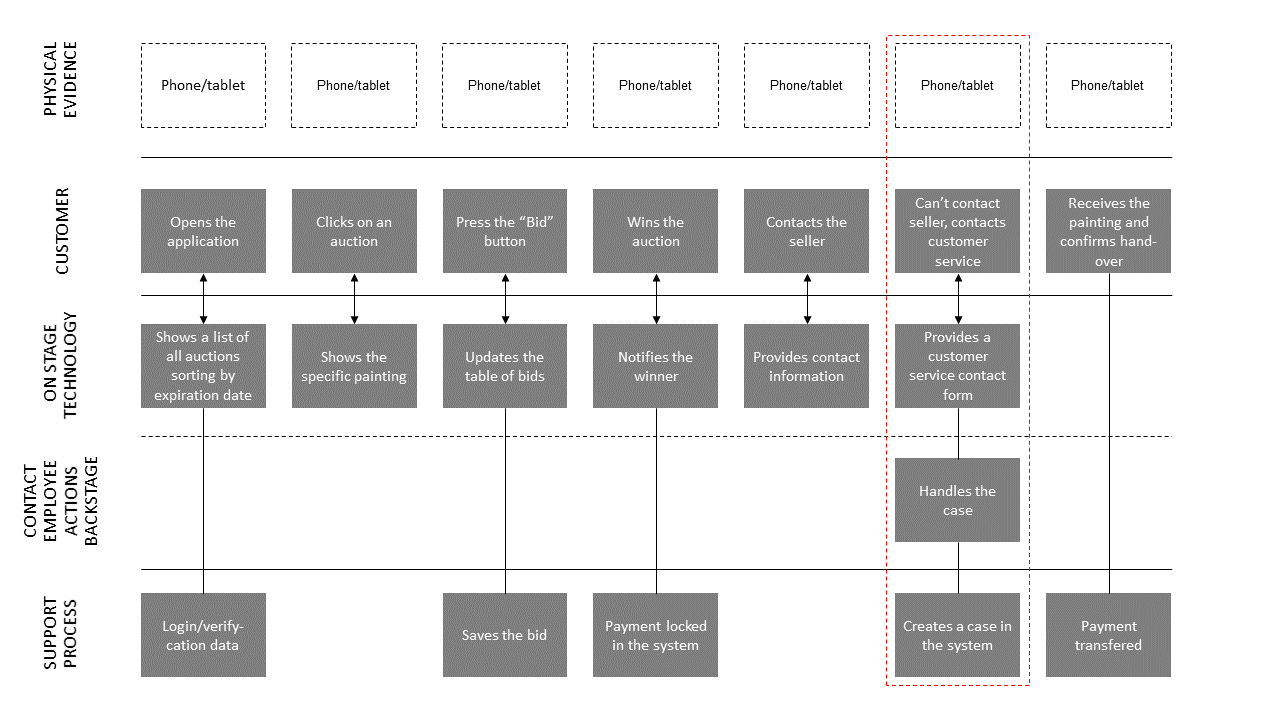
\includegraphics[angle=270,origin=c,width=13cm]{Appendix/BlueprintBuyer.PNG}
\label{ServiceBlueprintBuyer}
\end{figure}

\section{Screenshot of the auction-grid in the vertical prototype}
\label{AppScreenshots}
\begin{figure}[H]
    \centering
\caption{The grid displaying auctions}
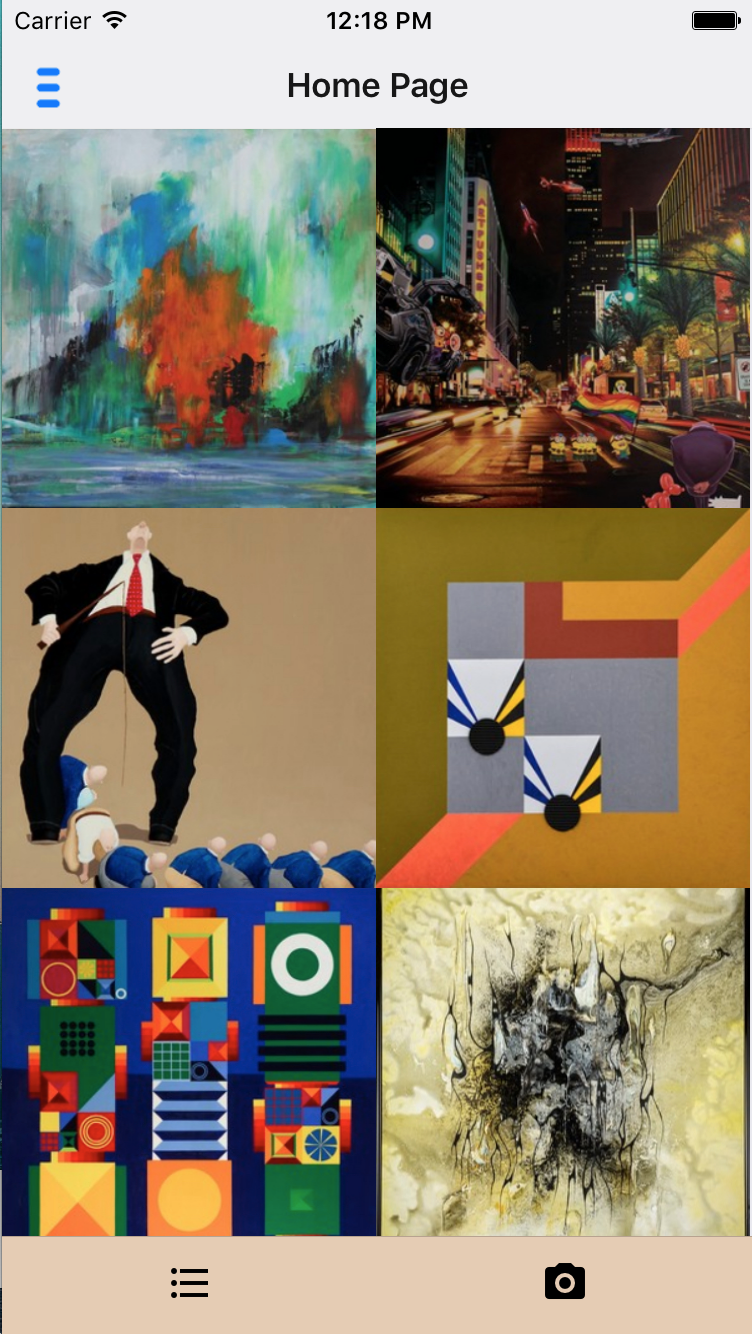
\includegraphics[width=8cm]{Appendix/Grid.png}
\label{AuctionsGrid}
\end{figure}
\newpage

\section{The two domains}
\label{Two domians}
\begin{center}
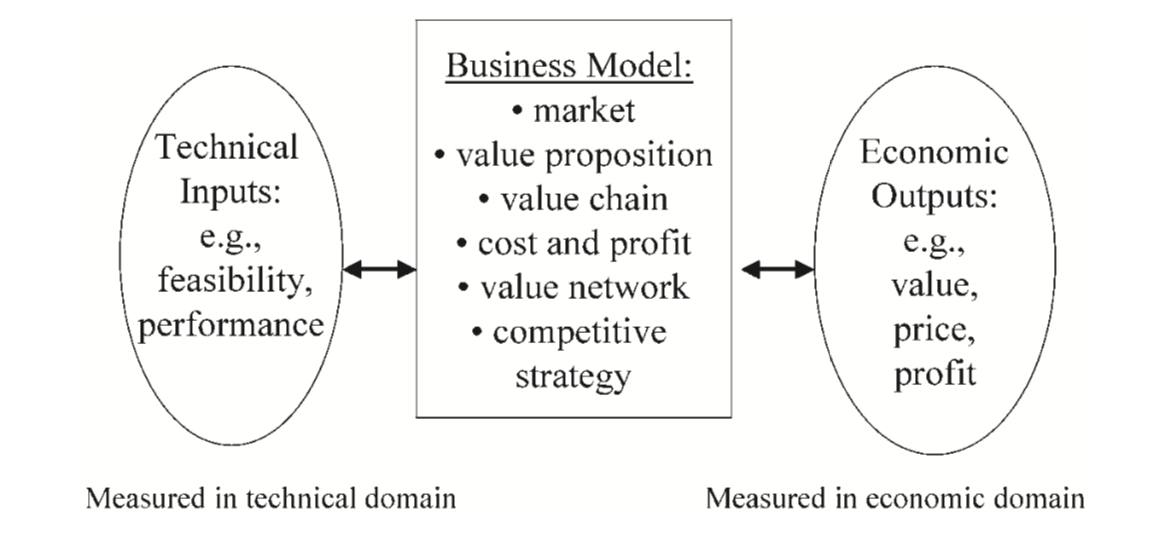
\includegraphics[width=14cm]{Appendix/twodomains.png}
\end{center}
\newpage
\section{Business models}
\label{BusinessModels}
The table below states the business model of Artion and the competitors. 

\begin{center}
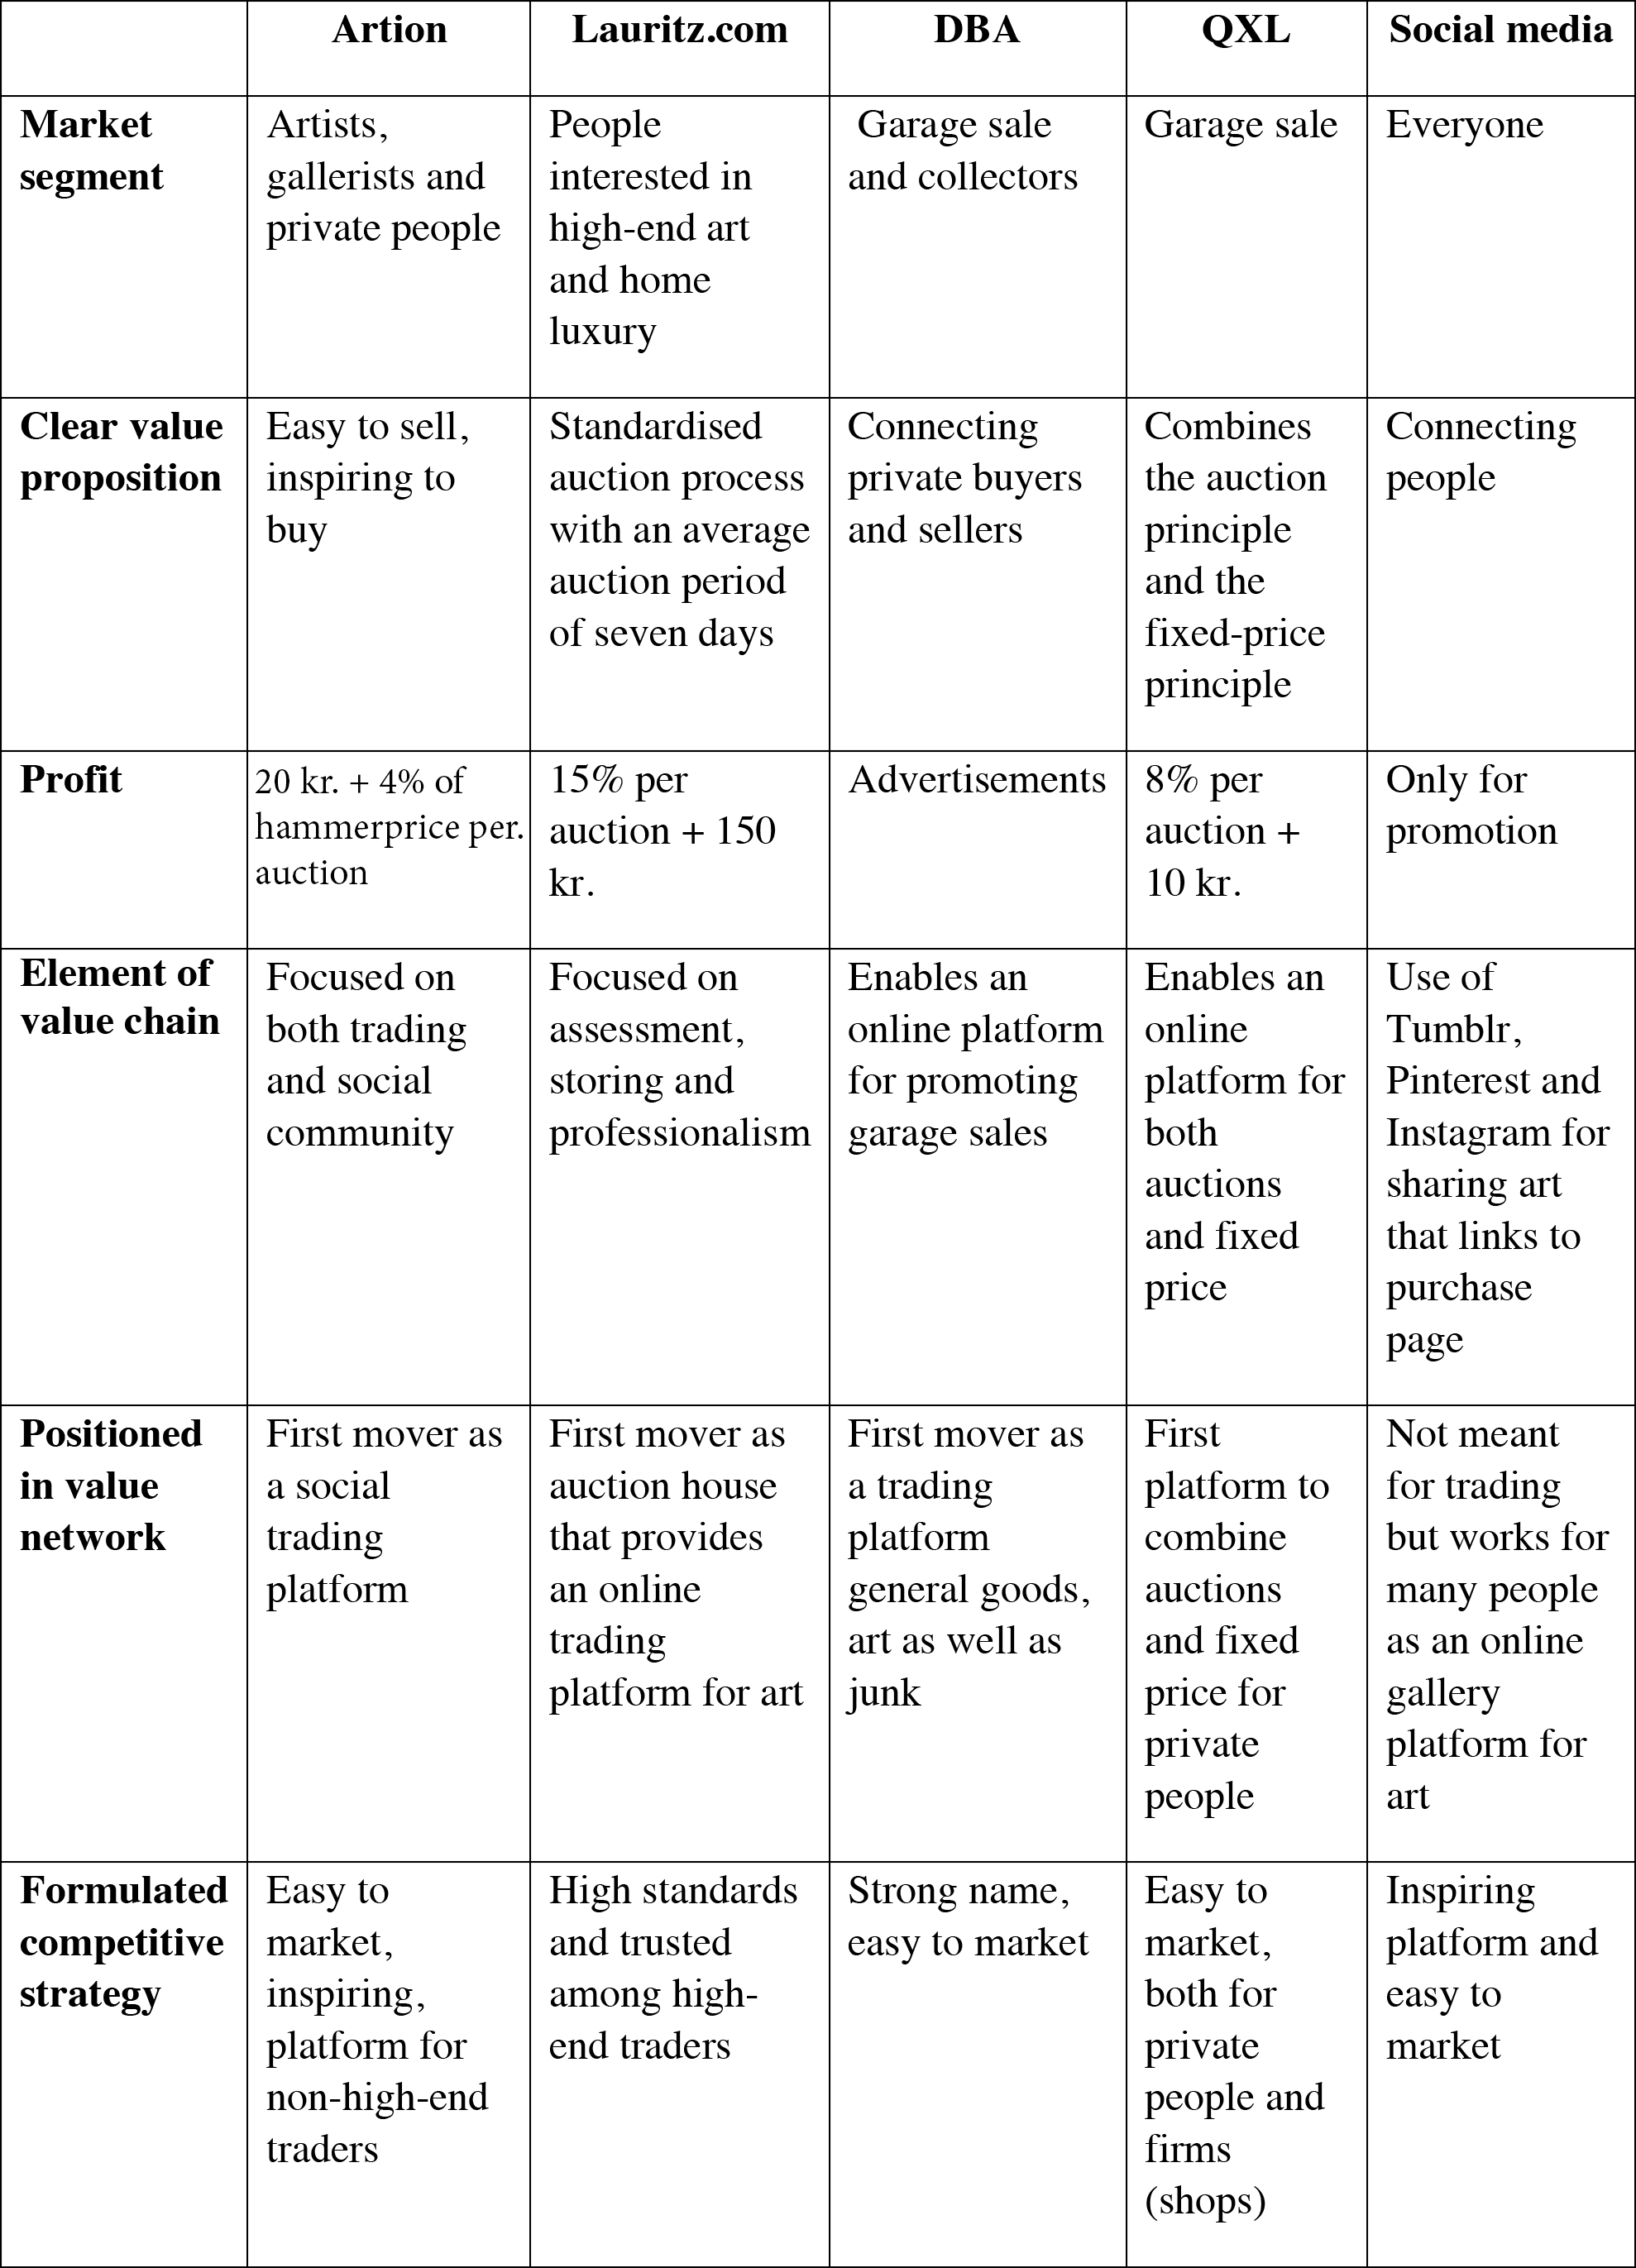
\includegraphics[width=15cm]{Appendix/BusinessModelsV2.png}
\end{center}

\section{Horizontal prototype}
\label{HorizontalPrototype}
\begin{figure}[H]
\centering
  \begin{minipage}[b]{0.31\linewidth}
    \caption{Auctions feed}
    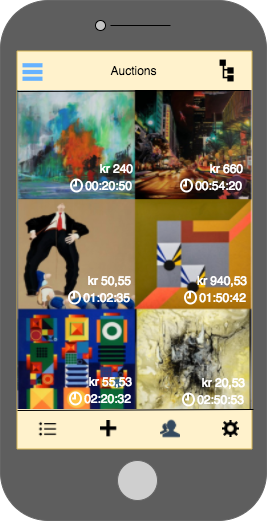
\includegraphics[width=\linewidth]{Appendix/HorizontalPrototype/1.png}
    \label{AuctionsFeed}
  \end{minipage}
  \hspace{1cm}
  \begin{minipage}[b]{0.31\linewidth}
    \caption{Personal gallery}
    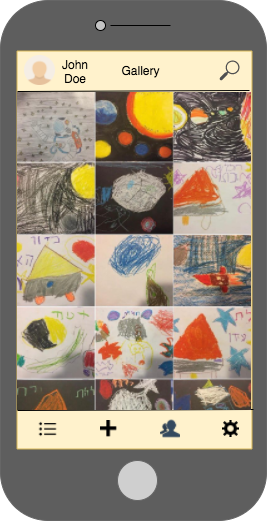
\includegraphics[width=\linewidth]{Appendix/HorizontalPrototype/2.png}
    \label{PersonalGallery}
  \end{minipage}
\end{figure}

\begin{figure}[H]
\centering
  \begin{minipage}[b]{0.31\linewidth}
    \caption{Menu}
    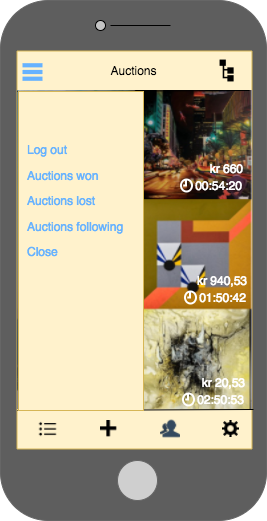
\includegraphics[width=\linewidth]{Appendix/HorizontalPrototype/3.png}
    \label{MainMenu}
  \end{minipage}
  \hspace{1cm}
  \begin{minipage}[b]{0.31\linewidth}
    \caption{\newline Confirmation interface}
    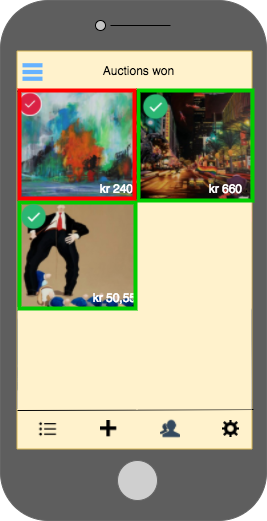
\includegraphics[width=\linewidth]{Appendix/HorizontalPrototype/4.png}
    \label{ConfirmationInterface}
  \end{minipage}
\end{figure}

\begin{figure}[H]
    \centering
\caption{The process of creating an auction}
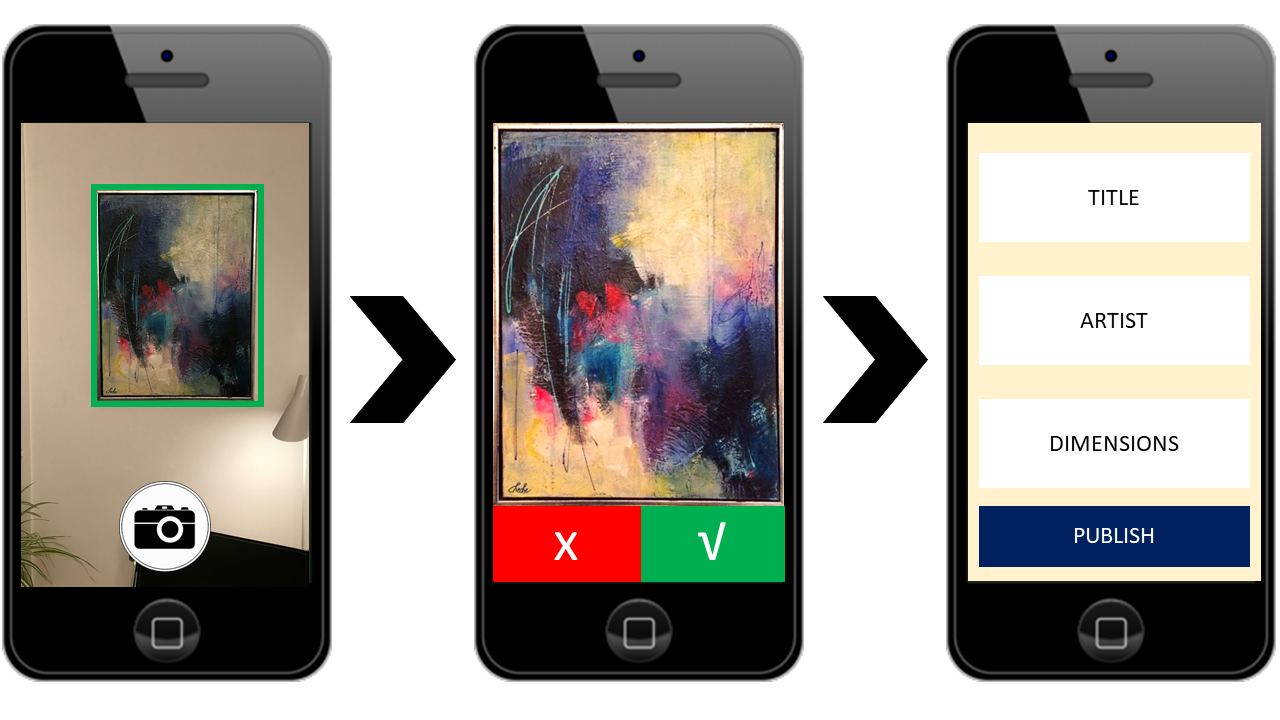
\includegraphics[width=16cm]{Appendix/HorizontalPrototype/5.png}
\label{CreateAuction}
\end{figure}




\section{Task-Focused Interface}
\label{TaskFocusedInterface}
\begin{figure}[H]
    \centering
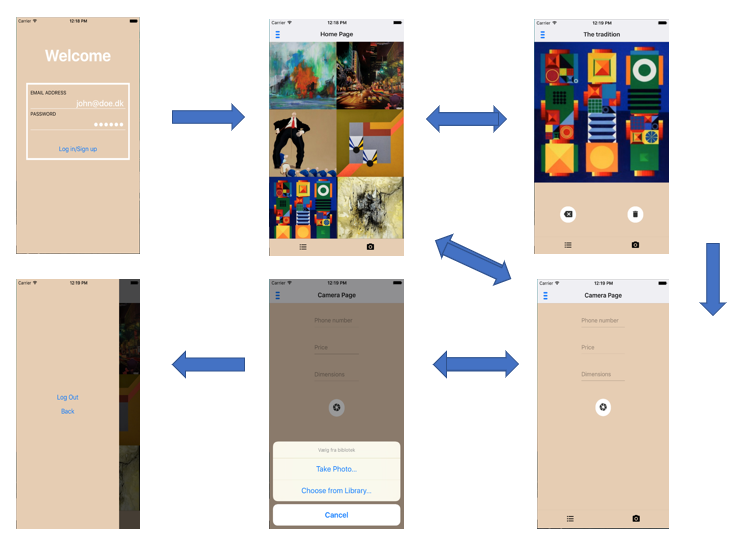
\includegraphics[width=16cm]{Appendix/TFI.png}
\label{TFI}
\end{figure}

\section{Commercial Challenges}
\label{CommercialChallenges}
\begin{center}
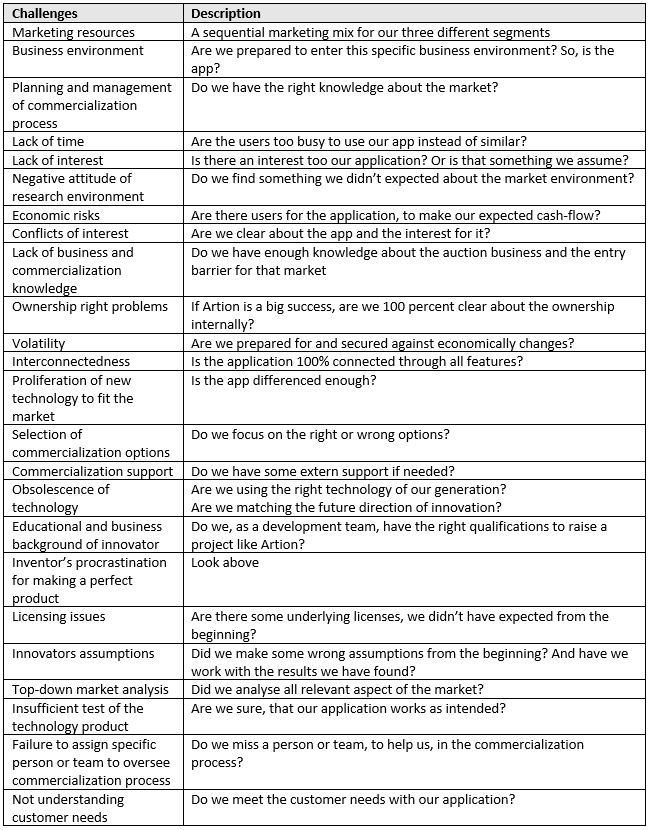
\includegraphics[width=15cm]{Appendix/CommercialChallenges.PNG}
\label{CommercialChallenges}
\end{center}

\section{Personas}
\label{Personas}
\subsubsection*{Persona 1: Artist}
- Personal information: Kjeld Andersen, age 34, Artist. Educated artist at 'Det Jyske Kunstakademi'. Works as a self-employed artist. Currently lives in Copenhagen Oe., together with his wife and two years old daughter.

- Needs: Kjeld could becoming a future user of our applications, as he want to scale the amount of potential buyers of his arts

- Motivation: The amount of users of our platform. The cheap fees and secure payment.

- Challenges: The current challenges that Kjeld faces, is that he doesn't hit many buyers, then he takes his art to the local vernissage. We can support Kjeld, by aiming a lot of direct and indirect buyers with our online platform.

- Buying role: He is the seller on this trading platform

\subsubsection{Persona 2: Gallerist}
- Personal information: Mogens Hermann, age 53, Gallerist. Educated Master of Fine Arts at "Det kongelige danske kunstakademi - billedkunstskolerne". Works at his own gallery. Currently lives in Copenhagen N., but have gained a lot of knowledge with his work in Los Angeles. 

- Needs: As Persona 1, he wants a platform, where he can hit a large amount of buyers, without any associations with DBA, Facebook or something else. 

- Motivation: Large number of potential buyers. Cheap fees. 

- Challenges: Doesn't hit many buyers. Our app supports the future by increase the amount of users

- Buying role: He is the seller on this trading platform.

\subsubsection{Persona 3: Private People}
- Personal information: Emma Jensen, age 24, art enthusiast. Educated pedagogue at 'Campus Carlsberg'. Works as an pedagogue at 'Skolen ved Søerne'. Currently lives in Amager with her boyfriend.

- Needs: She wants an application exclusively for paintings.

- Motivation: Cheap paintings. User friendly application. 

- Challenges: Too many opportunities for trading platforms. But not one specific for painting. 

- Buying role: She is the buyer on this trading platform.

\section{Vertical prototype}
\label{FullVerticalPrototype}
Screenshots of the main features in the vertical prototype.

\begin{figure}[H]
\centering
  \begin{minipage}[b]{0.285\linewidth}
    \caption{Login}
    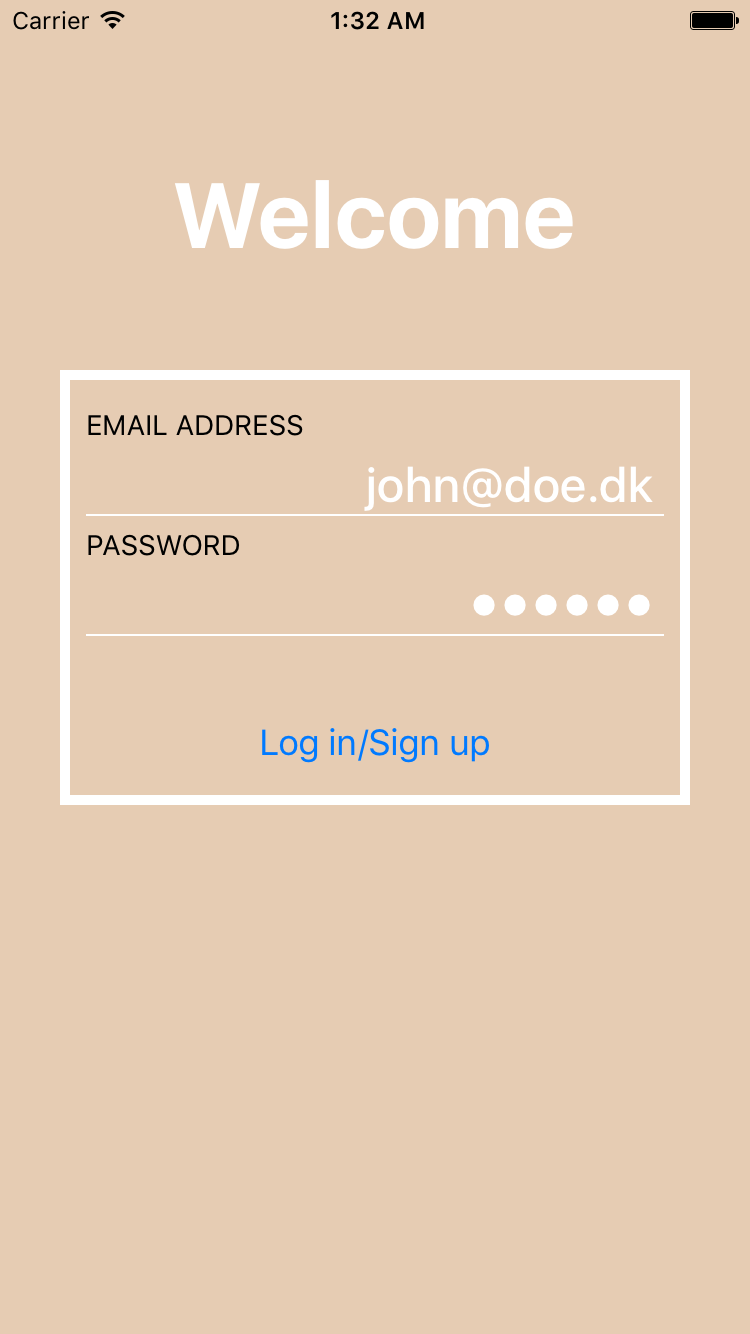
\includegraphics[width=\linewidth]{Appendix/VerticalPrototype/login.png}
  \end{minipage}
  \hspace{0.6cm}
  \begin{minipage}[b]{0.285\linewidth}
    \caption{Auctions grid}
    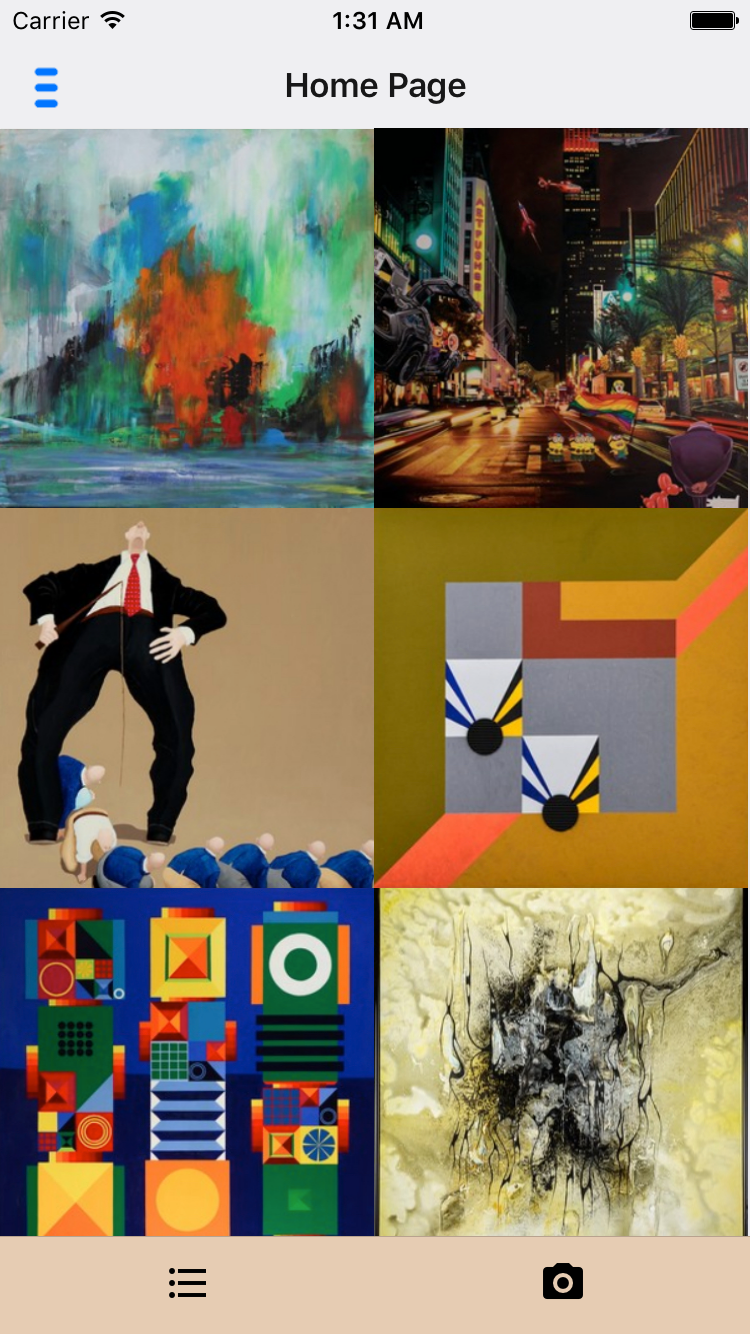
\includegraphics[width=\linewidth]{Appendix/VerticalPrototype/grid.png}
  \end{minipage}
 \hspace{0.6cm}
  \begin{minipage}[b]{0.285\linewidth}
    \caption{Menu}
    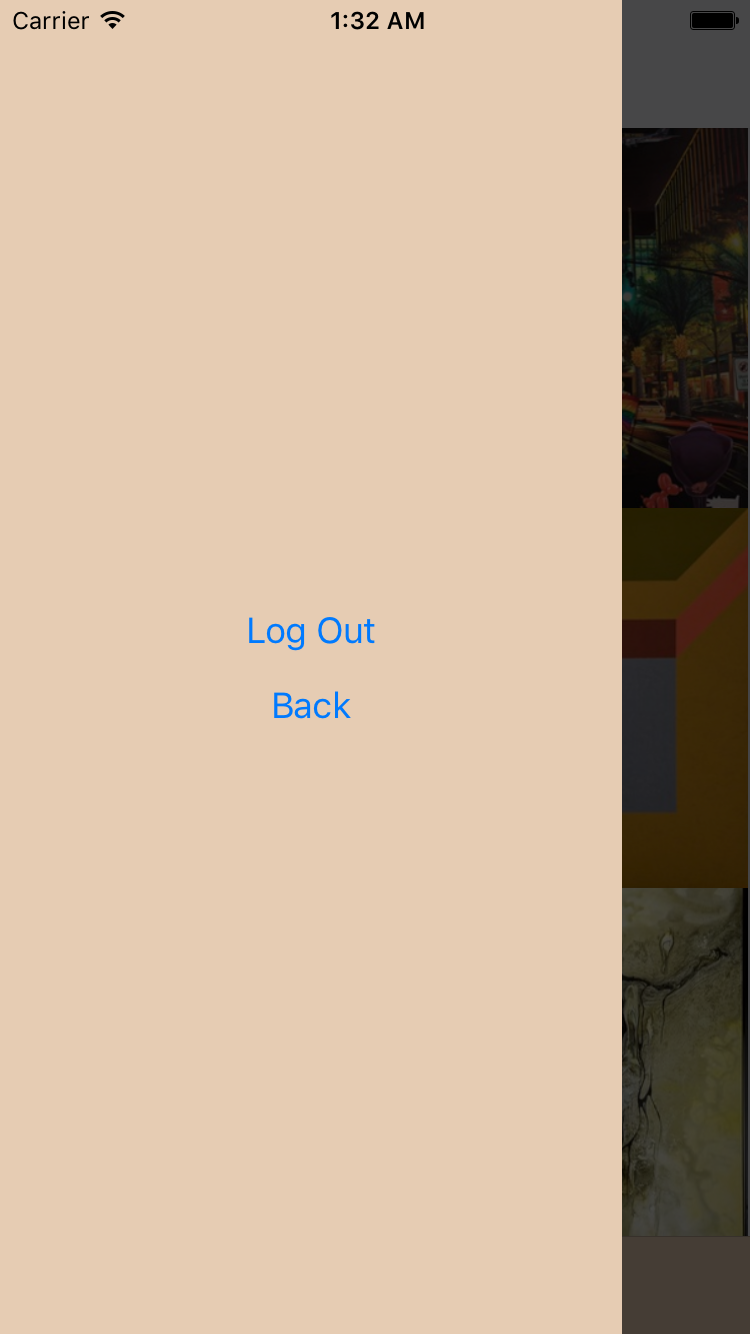
\includegraphics[width=\linewidth]{Appendix/VerticalPrototype/menu.png}
  \end{minipage}
\end{figure}

\begin{figure}[H]
\centering
  \begin{minipage}[b]{0.285\linewidth}
    \caption{Auction}
    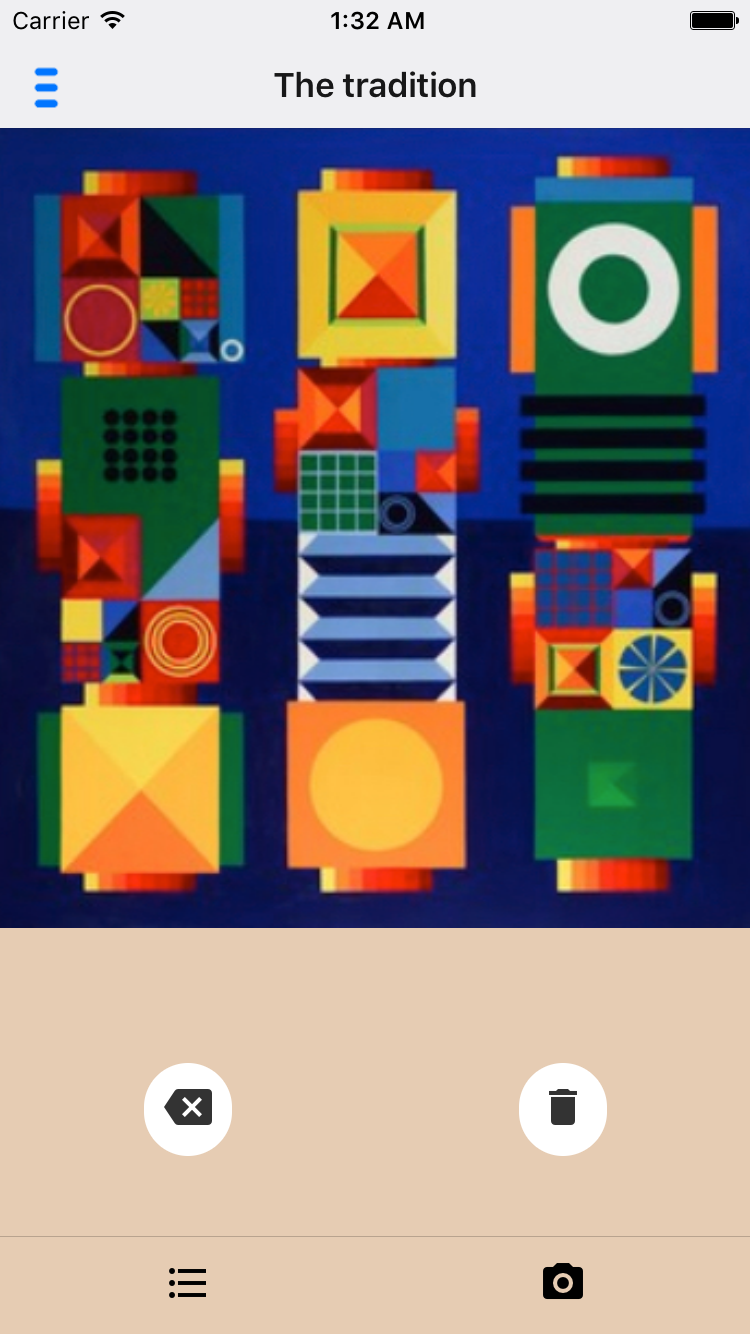
\includegraphics[width=\linewidth]{Appendix/VerticalPrototype/auction.png}
  \end{minipage}
  \hspace{0.6cm}
  \begin{minipage}[b]{0.285\linewidth}
    \caption{\newline Create auction}
    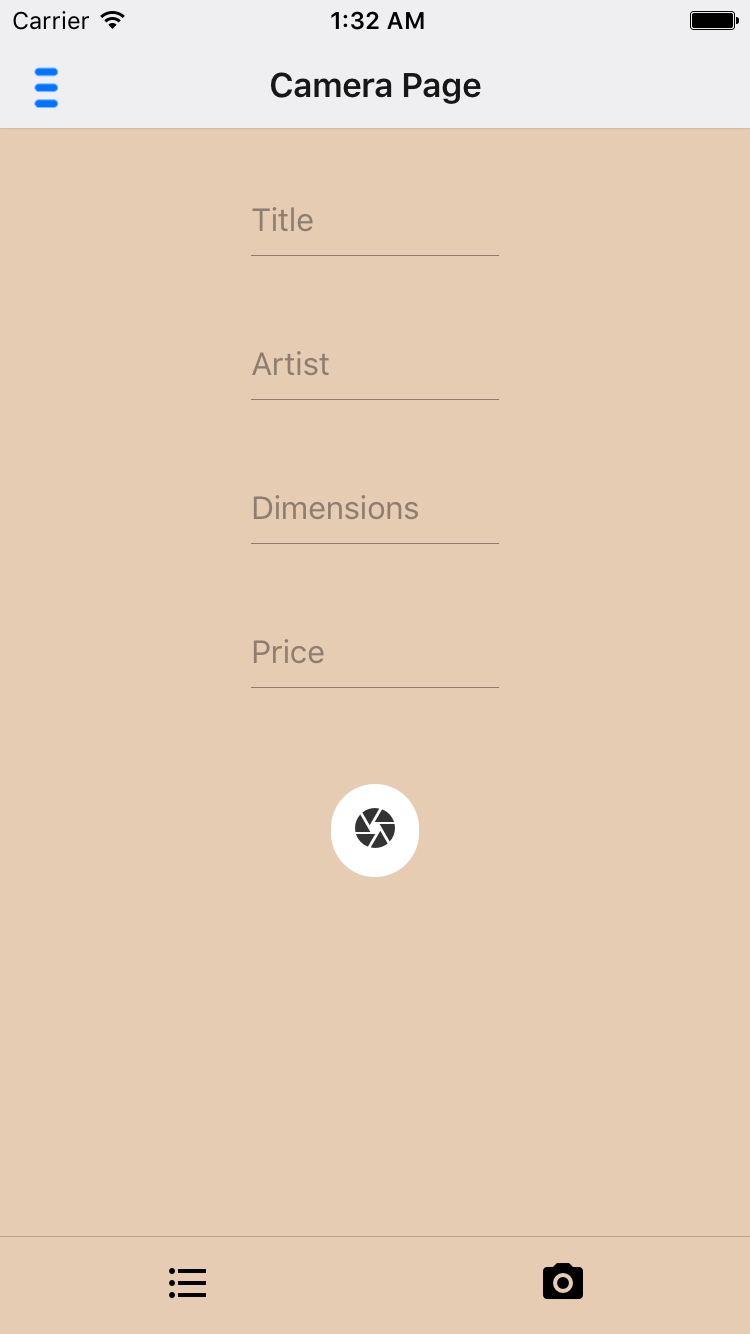
\includegraphics[width=\linewidth]{Appendix/VerticalPrototype/attributes.png}
  \end{minipage}
\end{figure}

\end{document}